\documentclass[11pt,aspectratio=169]{beamer}

\usepackage{slides}
\usepackage{soul}
\usepackage{pdfpc}
\usepackage{ebproof}
\usepackage{bigdelim}
\usepackage{booktabs}
\usepackage{listings}
\usepackage{tcolorbox}
\usepackage{tabularx}
\usepackage{tikz}
\usepackage{xspace}
\usepackage[T1]{fontenc}
\usepackage[utf8]{inputenc}
\usepackage[symbol]{footmisc}
\usepackage[noend]{algpseudocode}
\usepackage[
    backend    = biber,
    style      = alphabetic,
    giveninits = true,
    maxnames   = 16,
    minnames   = 16,
]{biblatex}

\addbibresource{./references.bib}

\usetikzlibrary{
    positioning,
    shapes.symbols,
    shadows,
    arrows,
    calc
}

\newcommand{\senc}{\text{senc}}
\newcommand{\msg}{\text{msg}}
\newcommand{\nonce}{\text{nonce}}
\newcommand{\KDF}{\text{KDF}}
\newcommand{\key}{\text{key}}

\newcommand{\Tamarin}[1]{\textsc{Tamarin}\xspace}

%% Print: [#1] -[#2]-> [#3]
\newcommand{\MSR}[3]{#1 -\hspace{-4pt}[\hspace{5pt} #2 \hspace{4pt}]\hspace{-4.6pt}\rightarrow #3}
%% Print: -[#1]->
\newcommand{\ActionFact}[1]{-\hspace{-4pt}[\hspace{5pt} #1 \hspace{4pt}]\hspace{-4.6pt}\rightarrow}
%% Print: ~
\newcommand{\tildelow}{\raisebox{0.5ex}{\texttildelow}}
%% Print: ^
\newcommand{\pow}{\textasciicircum{}}
%% Highlight text in overlay
\newcommand{\althl}[2][2]{\alt<#1>{\hl{#2}}{#2}}

%% Sticky notes to represent facts
\definecolor{StickyNoteYellow}{RGB}{241,239,161}
\definecolor{StickyNoteRed}{RGB}{255,167,169}
\definecolor{StickyNoteGreen}{RGB}{148,199,146}
\definecolor{StickyNoteBlue}{RGB}{167,229,241}
\NewDocumentCommand{\StickyNote}{O{StickyNoteYellow}O{1cm}m}{%
    \begin{tikzpicture}
        \node[
            drop shadow={
                shadow xshift = 2pt,
                shadow yshift = -4pt,
            },
            xslant = -0.1,
            yslant = 0.1,
            draw   = black,
            fill   = #1,
            text   = black,
        ] {\parbox[t][#2][c]{#2}{\centering#3}};
    \end{tikzpicture}
}

%% Colors for terms and facts
\definecolor{TermBlue}{HTML}{1C377D}
\definecolor{FactPurple}{HTML}{7C3655}

\newcommand{\term}[1]{\textcolor{TermBlue}{#1}}
\newcommand{\Term}[1]{\textcolor{TermBlue}{#1}}
\newcommand{\Fact}[1]{\textcolor{FactPurple}{#1}}

%% Other colors
\definecolor{AdversaryRed}{HTML}{DA3B26}

%% Listings
\lstset{escapeinside={(*@}{@*)}}
\lstset{numberstyle=\tiny}

\definecolor{TamarinBlue}{RGB}{42,0,255}
\definecolor{TamarinGreen}{RGB}{48,110,32}
\definecolor{TamarinPurple}{RGB}{175,36,67}

\lstdefinestyle{tamarin}{
    basicstyle    = \linespread{0.75}\footnotesize\ttfamily,
    extendedchars = true,
    tabsize       = 2,
    columns       = fixed,
    numbers       = none,
    breaklines    = true,
    literate      = {~}{{\raisebox{0.5ex}{\texttildelow}}}{1},
    morekeywords  = {theory, builtins, restriction, equations, functions, rule,
                     let, in, lemma, All, Ex, not, predicates, begin, end},
    keywordstyle  = \color{TamarinPurple},
    morecomment   = [l]{//},
    morecomment   = [s]{/*}{*/},
    commentstyle  = \color{TamarinGreen},
    xleftmargin   = 0mm,
    upquote       = true,
    morestring    = *[b]",
    showstringspaces = false
}

\lstdefinestyle{tactic}{
    basicstyle    = \linespread{0.75}\footnotesize\ttfamily,
    extendedchars = true,
    tabsize       = 2,
    columns       = fixed,
    numbers       = none,
    breaklines    = true,
    literate      = {~}{{\raisebox{0.5ex}{\texttildelow}}}{1},
    alsoletter    = :,
    morekeywords  = {tactic:, presort:, prio:, deprio:},
    keywordstyle  = \color{TamarinPurple},
    morecomment   = [l]{//},
    morecomment   = [s]{/*}{*/},
    commentstyle  = \color{TamarinGreen},
    xleftmargin   = 0mm,
    upquote       = true,
    morestring    = *[b]",
}

\lstdefinestyle{oracle}{
    basicstyle    = \linespread{0.75}\footnotesize\ttfamily,
    extendedchars = true,
    tabsize       = 2,
    columns       = fixed,
    numbers       = none,
    breaklines    = true,
    literate      = {~}{{\raisebox{0.5ex}{\texttildelow}}}{1},
    morecomment   = [l]{\#},
    morekeywords  = {import, for, in, if, elif},
    keywordstyle  = \color{TamarinPurple},
    commentstyle  = \color{TamarinGreen},
    xleftmargin   = 0mm,
    upquote       = true,
}

\definecolor{ProVerifGreen}{RGB}{48,110,32}
\definecolor{ProVerifBlue}{RGB}{64,112,161}

\lstdefinestyle{proverif}{
    basicstyle    = \linespread{0.75}\footnotesize\ttfamily,
    extendedchars = true,
    tabsize       = 2,
    columns       = fixed,
    numbers       = none,
    breaklines    = true,
    literate      = {~}{{\raisebox{0.5ex}{\texttildelow}}}{1},
    morecomment   = [s]{(*}{*)},
    commentstyle  = \color{ProVerifGreen},
    keywordstyle  = \color{ProVerifBlue},
    morekeywords  = {in, if, event, new, let, out},
    xleftmargin   = 0mm,
}

\definecolor{proofTreeBlue}{HTML}{2639B0}
\definecolor{proofTreeRed}{HTML}{921C12}

\lstdefinestyle{prooftree}{
    basicstyle    = \linespread{0.8}\footnotesize\fontfamily{pcr}\selectfont,
    extendedchars = true,
    tabsize       = 2,
    columns       = fixed,
    numbers       = left,
    breaklines    = true,
    literate      = {~}{{\raisebox{0.5ex}{\texttildelow}}}{1},
    keywords      = [1]{lemma, case, next, qed, by, end, Diff-Lemmas},
    keywordstyle  = [1]\color{black}\bfseries,
    keywords      = [2]{simplify, solve, sorry, contradiction, induction,
                        autoprove, rule-equivalence},
    keywordstyle  = [2]\color{proofTreeBlue}\bfseries,
    keywords      = [3]{@, \|, <, \^},
    keywordstyle  = [3]\color{proofTreeRed},
    alsoletter    = @\|<\^-,
    moredelim     = **[is][{\color{proofTreeBlue}}]{<<}{>>},
    xleftmargin   = 0mm,
    upquote       = true,
    morestring    = *[b]",
}

%% Color boxes
\definecolor{ColorBoxBlue}{HTML}{1C377D}
\tcbset{
    colback      = white,
    colframe     = black,
    fonttitle    = \bfseries,
    coltitle     = white,
    colbacktitle = ColorBoxBlue,
    boxrule      = 1pt
}

%% Vertical separator for frames
\newcommand<>{\vsep}{
    \begin{tikzpicture}[remember picture,overlay]%
        \draw[ultra thick]
            ($(current page.north west)+(8cm,0.5cm)$) to
            ($(current page.south west)+(8cm,-0.5cm)$)
        ;
    \end{tikzpicture}%
}

%% Horizontal separator for frames
\newcommand<>{\hsep}{
    \begin{tikzpicture}[remember picture,overlay]%
        \draw[ultra thick]
            ($(current page.north west)+(-0.5cm,-4.5cm)$) to
            ($(current page.north east)+(0.5cm,-4.5cm)$)
        ;
    \end{tikzpicture}%
}


\title{Formal Analysis of Real-World Security Protocols}
\subtitle{Lecture 2: Protocols in the Symbolic Model}
\date{\today}
\author{Aleksi Peltonen}
\institute{CISPA Helmholtz Center for Information Security}

\begin{document}
\maketitle

% ---------------------------------------------------------------------------- %
% Content
% ---------------------------------------------------------------------------- %

\begin{frame}[fragile]{Recap: Terms}
    \begin{columns}
        \begin{column}[c]{0.5\textwidth}
            \begin{itemize}
                \item \textbf{Terms} are recursively constructed from
                      \textit{constants}, \textit{variables}, and
                      \textit{function symbols}
                \item They represent messages by the way they were constructed
                \item Each \textbf{subterm} $s|_p$ of $t$ has a unique
                      \textbf{position}, e.g.,
                \begin{itemize}
                    \item $s|_{[1]} = $ <msg, nonce>
                    \item $s|_{[2,1]} = $ K
                \end{itemize}
            \end{itemize}
        \end{column}
        \begin{column}[c]{0.5\textwidth}
            \begin{figure}
                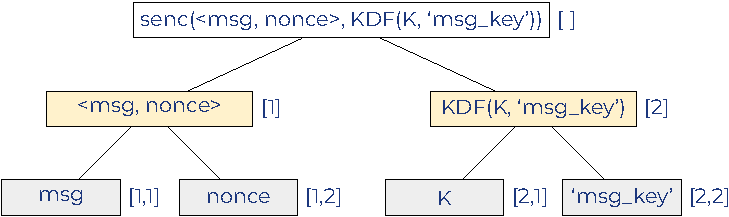
\includegraphics[width=1.05\textwidth]{figures/lecture_2/terms}
            \end{figure}
        \end{column}
    \end{columns}
    \vsep
\end{frame}

\begin{frame}[fragile]{Recap: Term rewriting}
    \begin{itemize}
        \item Terms can contain \textbf{variables}
        \begin{itemize}
            \item e.g., $t_1$ = senc(<msg, nonce>, \textbf{X})
        \end{itemize}
        \item A \textbf{substitution} is a mapping
              $\sigma: \mathcal{V} \rightarrow \mathcal{T}$
              that replaces variables with terms
        \begin{itemize}
            \item We can apply the substitution
                $\sigma = \{\text{X} \mapsto \KDF(\text{K},$`$\msg\_\key$'$)\}$ 
                to get $t_2 = t_1\sigma =$
                senc(<\msg, \nonce>, \KDF(K, `\msg\_\key')).
        \end{itemize}
        \item A \textbf{rewrite rule} $l \rightarrow r$ can be applied on a 
              term if it has a subterm that matches $l$. The operation replaces 
              $l$ with $r$
        \begin{itemize}
            \item We can apply the rewrite rule
                  $KDF(Y,Z) \rightarrow \mathit{SessionKey}$
                  and the substitution
                  $\sigma = \{\text{Y} \mapsto \text{K}, \text{Z}
                  \mapsto $`$\msg\_\key$'$\}$ on $t_2$ to get \\
                  $t_3$ = senc(<msg, nonce>, SessionKey)
        \end{itemize}
    \end{itemize}
\end{frame}

\begin{frame}[fragile]{Recap: Equational theories}
    \begin{itemize}
        \item A \textbf{signature} $\Sigma$ is a set of
              \textbf{function symbols}, each with an \textit{arity}
        \begin{itemize}
            \item Function symbols of arity 0 are called \textbf{constants}
        \end{itemize}
        \item An \textbf{equation} over the signature $\Sigma$ is a pair of 
              terms $s,t \in \mathcal{T}_{\Sigma}(\mathcal{V})$ that defines 
              when the terms are considered equal
        \begin{itemize}
            \item Instead of modeling exponentiation, we use an equation to 
                  define the expected equality:
                  (X\pow{}Y)\pow{}Z = (X\pow{}Z)\pow{}Y
        \end{itemize}
        \item An \textbf{equational theory} is a tuple $(\Sigma, E)$ of a 
              signature $\Sigma$ and a set of equations $E$
    \end{itemize}
\end{frame}

\begin{frame}[fragile]{Model components}
    What \textbf{components} do we need to model protocols?

    \begin{table}
        \raggedright
        \begin{tabular}{lll}
            1. & All possible sent and received messages
               & \rdelim\}{1}{3mm}[\hspace*{3mm}Lecture 1] \\[.2cm]
            2. & All possible protocol behaviors
               & \rdelim\}{1}{3mm}[\hspace*{3mm}\hl{Lecture 2}] \\[.2cm]
            3. & The attacker
               & \rdelim\}{2.2}{3mm}[\hspace*{2mm}Lecture 3] \\[.2cm]
            4. & Security properties that we want to verify
        \end{tabular}
    \end{table}
\end{frame}

\begin{frame}[fragile]{This lecture}
    \tableofcontents
\end{frame}

% ---------------------------------------------------------------------------- %

\section{Unification}

% ---------------------------------------------------------------------------- %

\begin{frame}[fragile]{Unification modulo E}
    Recall from last week: \textbf{Unification} determines if two terms with 
    variables can be made equal. Two terms $s$ and $t$ are said \textit
    {unifiable} if there exists a substitution $\sigma$, called a \textit
    {unifier}, such that $s\sigma = t\sigma$.\\[.3cm]

    In practice, we often perform unification \textbf{modulo} $E$, i.e., taking 
    into account some equational theory. We write this as $=_E$.

    \begin{tcolorbox}[title=Example]
        The equation $x \times 1 = y \times 2$ has no solution if we only 
        consider only syntactic equality, since we have not defined anything 
        about the multiplication function. However, if we define
        \textit{commutativity} for the operator, we can solve the equation 
        using e.g., $\sigma = \{x \mapsto 2, y \mapsto 1\}$.
    \end{tcolorbox}
\end{frame}

% ---------------------------------------------------------------------------- %

\section{Term Deduction}

% ---------------------------------------------------------------------------- %

\begin{frame}[fragile]{Inference rules}
    \begin{itemize}
        \item An \textbf{inference rule} is of the form:
        \begin{equation*}
            \begin{prooftree}
                \hypo{t_1}
                \hypo{t_2}
                \hypo{\cdots}
                \hypo{t_n}
                \infer4{t}
            \end{prooftree}
        \end{equation*}
        where $t$ and $t_1, \dots, t_n$ are terms
        \item Defines how we can use a set of terms to learn a new term
        \item An \textbf{inference system} is a set of inference rules
        \item We can use inference rules to represent
              \textbf{attacker capabilities} in our model!
        \begin{itemize}
            \item More in lecture 3, when we talk about attacker models
        \end{itemize}
    \end{itemize}
\end{frame}

\begin{frame}[fragile]{Term deduction}
    \begin{itemize}
        \item What can we deduce from the knowledge we have?
        \item \textbf{Deduction rules:}
            \begin{enumerate}
                \item Construction:
                    \begin{equation*}
                        \begin{prooftree}
                            \hypo{k}
                            \hypo{m}
                            \infer2{\senc(m, k)}
                        \end{prooftree}
                    \end{equation*}
                \item Deconstruction:
                    \begin{equation*}
                        \begin{prooftree}
                            \hypo{k}
                            \hypo{\senc(m, k)}
                            \infer2{m}
                        \end{prooftree}
                    \end{equation*}
            \end{enumerate}
        \item More in lecture 4, when we talk about constraint systems
    \end{itemize}
\end{frame}

\begin{frame}[t]{Term deduction example}
    Let $\mathcal{T}$ be a set of terms as follows:
    {\setbeamercolor{alerted text}{fg=red}
    \begin{equation*}
        \mathcal{T} = \{
            \alert<2>{\senc(a, b)},
            \alert<3>{\senc(b, c)},
            \alert<4>{\senc(c, d)},
            \alert<5>{\langle d, e \rangle}
        \}
    \end{equation*}}
    \setbeamercovered{transparent}
    Can we deduce $a$? \only<2->{\textbf{Yes.}}
    \begin{equation*}
        \begin{prooftree}
            \only<-5>{}\hypo{\langle d, e \rangle}
            \only<-4>{\rewrite{}}\infer1{d}
            \only<-3>{\rewrite{}}\hypo{\senc(c, d)}
            \only<-3>{\rewrite{}}\infer2{c}
            \only<-2>{\rewrite{}}\hypo{\senc(b, c)}
            \only<-2>{\rewrite{}}\infer2{b}
            \only<-1>{\rewrite{}}\hypo{\senc(a, b)}
            \only<-1>{\rewrite{}}\infer2{a}
        \end{prooftree}
    \end{equation*}
\end{frame}

\begin{frame}[fragile]{Automatic term deduction}
    \begin{itemize}
        \item \textbf{Intruder deduction problem}:
              given a state of the protocol execution, can the intruder derive 
              a given message m?
        \item Is manual message deduction possible? \textbf{Yes.}
        \item Is it easy an convenient? \textbf{No.}
        \item Can we automate it? \textbf{Yes!}
        \item More in lecture 5, when we talk about \Tamarin's constraint 
              solving algorithm
    \end{itemize}
\end{frame}

% ---------------------------------------------------------------------------- %

\section{Protocol Modeling}

% ---------------------------------------------------------------------------- %

\begin{frame}[fragile]{Modeling protocol execution}
    \begin{columns}
        \begin{column}{0.6\textwidth}
            Protocol descriptions are ``blueprints'':
            \begin{itemize}
                \item Protocols describe multiple  \textbf{roles}
                \begin{itemize}
                    \item e.g., client - server, initiator - responder
                \end{itemize}
                \item Parties \textbf{execute} these roles
                \begin{itemize}
                    \item e.g., Alice as the initiator, Bob as the responder, 
                          Charlie as the client, etc.
                    \item Parties can execute multiple roles
                    \item Each role execution at a party is a separate
                          \textbf{thread}
                \end{itemize}
            \end{itemize}
        \end{column}
        \begin{column}[c]{0.4\textwidth}
            \begin{figure}
                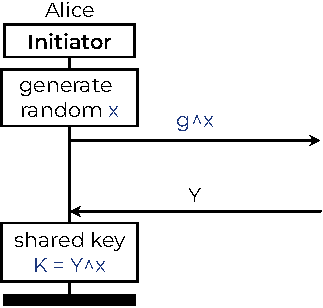
\includegraphics[width=\textwidth]{./figures/lecture_2/dh_a}%
            \end{figure}
        \end{column}
    \end{columns}
\end{frame}

\begin{frame}[fragile]{Modeling protocols}
    \begin{columns}
        \begin{column}{0.5\textwidth}
            \begin{itemize}
                \item By now you have seen how to model messages as terms:
                \begin{itemize}
                    \item We represent cryptographic functions with
                          \textbf{equational theories}
                    \item We can deduce terms from other terms
                \end{itemize}
                \item How do we combine all this to model protocols?
                \begin{itemize}
                    \item Multiple options!
                \end{itemize}
            \end{itemize}
        \end{column}
        \begin{column}{0.5\textwidth}
            \begin{onlyenv}<1>
                \begin{enumerate}
                    \item Modeling protocols as \textbf{processes}\\
                    (e.g., ProVerif)
                \end{enumerate}
                \vspace*{.5cm}
                \begin{lstlisting}[style=proverif,gobble=16]
                    let A(K:bitstring) =
                      new msg:bitstring;
                      out(c, (msg, HMAC(msg, K)));
                      event SendMessage(msg)
                    .

                    let B(K:bitstring) =
                      in(c, (msg:bitstring,
                             MAC:bitstring));
                      if MAC = HMAC(msg, K) then
                      event ReceiveMessage(msg)
                    .
                \end{lstlisting}
                \begin{tikzpicture}[remember picture, overlay]
                    \node[below left] at (current page.north east) {
                        
\includegraphics[width=0.15\textwidth]
                            {./figures/lecture_0/proverif_logo}
                    };
                    \node[above left, yshift=.3cm, xshift=-1.1cm]
                    at (current page.south east) {
                        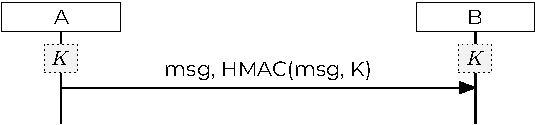
\includegraphics[width=.8\textwidth]
                            {./figures/lecture_0/protocol_2}%
                    };
                \end{tikzpicture}
            \end{onlyenv}%
            \begin{onlyenv}<2>
                \begin{enumerate}
                    \setcounter{enumi}{1}
                    \item Modeling protocols as
                          \textbf{multiset rewriting rules} (e.g., Tamarin)
                \end{enumerate}
                \vspace*{.5cm}
                \begin{lstlisting}[style=tamarin,gobble=16]
                    rule a_snd_msg:
                      [ !A(K)
                      , Fr(~msg) ]
                    --[ SendMessage(msg) ]->
                      [ Out(<~msg, HMAC(~msg,K)>) ]


                    rule b_rcv_msg:
                      [ !B(K)
                      , In(<msg, HMAC(msg, K)>) ]
                    --[ ReceiveMessage(msg) ]->
                      [ ]
                \end{lstlisting}
                \begin{tikzpicture}[remember picture, overlay]
                    \node[below left] at (current page.north east) {
                        
\includegraphics[width=0.15\textwidth]
                            {./figures/lecture_2/tamarin_logo_pixel}
                    };
                    \node[above left, yshift=.3cm, xshift=-1.1cm]
                    at (current page.south east) {
                        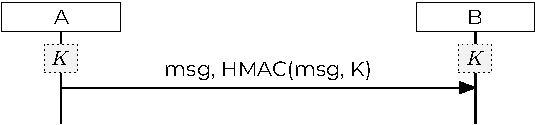
\includegraphics[width=.8\textwidth]
                            {./figures/lecture_0/protocol_2}%
                    };
                \end{tikzpicture}
            \end{onlyenv}
        \end{column}
    \end{columns}
    \vsep
\end{frame}

% ---------------------------------------------------------------------------- %

\section{Protocols as Rules and Facts}

% ---------------------------------------------------------------------------- %

\begin{frame}[fragile]{Facts}
    \begin{itemize}
        \item \Fact{\textbf{Facts}} are used to store information about
        \begin{enumerate}
            \item the transition system's current \textbf{state}
            \item the performed actions that are relevant for property 
                  specification
        \end{enumerate}
        \item Informally: \textit{sticky notes on a fridge}
        \vspace*{.5cm}
        \begin{figure}
            \StickyNote[StickyNoteYellow][1.8cm]{$\mathit{Key(k)}$}%
                \hspace*{.4cm}
            \StickyNote[StickyNoteBlue][1.8cm]{$\mathit{Id(Alice)}$}%
                \hspace*{.4cm}
            \StickyNote[StickyNoteGreen][1.8cm]{$\mathit{Msg(Hi)}$}%
                \hspace*{.4cm}
            \StickyNote[StickyNoteRed][1.8cm]{$\mathit{Secret(s)}$}%
        \end{figure}
    \end{itemize}
\end{frame}

\begin{frame}[fragile]{Facts}
    \begin{itemize}
        \item Formally: We assume an unsorted signature $\Sigma_{Fact}$ and 
              define a \textbf{fact} as F($t_1, \dots, t_n$) for
              F$\in \Sigma_{Fact}$ and $t_1, \dots, t_n \in \mathcal{T}_{\Sigma}
              (\mathcal{V \cup C})$
        \item We define the \textit{state} of the global transition system as a 
              \textbf{multiset of facts}
        \begin{itemize}
            \item A multiset (sometimes also called a ``bag'') is a set, in 
                  which members can occur multiple times
            \begin{itemize}
                \item e.g., $\{1,1,1,1,\dots\}$, $\{Alice, Alice, Bob\}$,
                            $\{a, a, b, c, d, d, e\}$
            \end{itemize}
            \item We write $\subseteq^{\sharp}$ for multiset inclusion,
                  $\cup^{\sharp}$ for multiset union, and
                  $\smallsetminus^{\sharp}$ for multiset difference
            \item $X^{\sharp}$ denotes the finite multisets with elements from 
                  $X$
        \end{itemize}
    \end{itemize}
\end{frame}

\begin{frame}[fragile]{Facts}
    \begin{itemize}
        \item Facts can be either \textbf{linear} or \textbf{persistent}
        \begin{itemize}
            \item Linear facts are consumed when we use them in a transition 
                  system
            \item Persistent fact do not change
        \end{itemize}
        \item Tamarin has several built-in fact symbols:
        \begin{table}[]
            \raggedright
            \begin{tabular}{lllll}
                \verb|K/1| &:& \verb|K(t)| & --
                    & check if the adversary can derive the term \verb|t| \\
                \verb|In/1| &:& \verb|In(t)| & --
                    & \verb|t| was received from the network \\
                \verb|Out/1| &:& \verb|Out(t)| & --
                    & \verb|t| was sent to the network \\
                \verb|Fr/1| &:& \verb|Fr(t)| & --
                    & \verb|t| was freshly generated
            \end{tabular}
        \end{table}
    \end{itemize}
\end{frame}

\begin{frame}[fragile]{Rules}
    \textbf{Rules} model the possible \textit{transitions} in a protocol.
    \begin{itemize}
        \item Syntax: $L \rightarrow R$
    \end{itemize}

    Intuitively, rules specify transitions as follows: If there is an 
    instantiation of the facts in $L$ in the current state of the system, we 
    can make a transition to replace the facts in $L$ by the facts in $R$ with 
    the same instantiation.

    \begin{tcolorbox}[title=Example]
        Consider a system state $S_n = [Msg(\text{`}hello\text{'})]$ and a rule 
        $Msg(X) \rightarrow Msg(Y)$. Using the substitution
        $\sigma = \{X \mapsto \text{`}hello\text{'}, Y \mapsto
        \text{`}bye\text{'}\}$ we can apply the rule to get
        $S_{n+1} = [Msg(\text{`}bye\text{'})]$.
    \end{tcolorbox}
\end{frame}

\begin{frame}[fragile]{Rules}
    We use rule in several different ways:
    \begin{itemize}
        \item \textbf{Adversary rules} determine which messages the adversary 
              can deduct from its knowledge set
        \item \textbf{Protocol} rules formalize the behavior of the model we 
              are analyzing
        \item \textbf{Initialization rules} define the generation of 
              cryptographic keys and other values
        \item \textbf{The \textsc{Fresh} rule} is a special built-in rule that 
              generates a unique (fresh) value
        \begin{itemize}
            \item Syntax: $[\;] \rightarrow [\,Fr(x)\,]$
        \end{itemize}
    \end{itemize}
\end{frame}

% ---------------------------------------------------------------------------- %

\section{Multiset Rewriting}

% ---------------------------------------------------------------------------- %

\begin{frame}[fragile]{Multiset rewriting (informally)}
    \begin{columns}
        \begin{column}{0.65\textwidth}
            \begin{itemize}
                \item Multiset rewriting
                \begin{itemize}
                    \item \Term{\textbf{Terms}}
                          (think ``messages'')
                    \item \Fact{\textbf{Facts}}
                          (think ``sticky notes on the fridge'')
                \end{itemize}
                \item The state of a system is a multiset of facts
                \begin{itemize}
                    \item Initial state is the empty multiset
                    \item Rules specify the transition rules (``moves'')
                \end{itemize}
                \item Rules are of the form:
                \begin{itemize}
                    \item $[\;\Fact{l}\;] \rightarrow [\;\Fact{r}\;]$ \quad
                          (or $\MSR{[\;\Fact{l}\;]}{\Fact{a}}{[\;\Fact{r}\;]}$)
                \end{itemize}
            \end{itemize}
        \end{column}
        \begin{column}{0.35\textwidth}
            \begin{figure}
                \StickyNote[StickyNoteYellow]{$F_1$}
                \StickyNote[StickyNoteGreen]{$F_2$}
                \StickyNote[StickyNoteRed]{$F_3$}\\[.5cm]
                    $[F_1, F_2] \rightarrow [F_4]$\\[.5cm]
                \StickyNote[StickyNoteRed]{$F_3$}
                \StickyNote[StickyNoteBlue]{$F_4$}
            \end{figure}
        \end{column}
    \end{columns}
    \begin{tikzpicture}[remember picture,overlay]%
        \draw[ultra thick]
            ($(current page.north west)+(10.1cm,0.5cm)$) to
            ($(current page.south west)+(10.1cm,-0.5cm)$);
    \end{tikzpicture}%
\end{frame}

\begin{frame}[fragile]{Multiset rewriting (formally)}
    \begin{itemize}
        \item We model the states of our transition system as finite
              \textbf{multisets of facts}
        \begin{itemize}
            \item We use a fixed set of fact symbols to encode the
                  \textit{adversary's knowledge},
                  \textit{freshness information}, and the
                  \textit{messages} on the network
            \item The remaining fact symbols are used to represent the protocol 
                  state
        \end{itemize}
        \item We assume an unsorted signature $\Sigma_{Fact}$ partitioned into 
              \textbf{linear} and \textbf{persistent} fact symbols
        \item We define the set of facts as the set $\mathcal{F}$ consisting of 
              all facts $F(t_1, .., t_k)$ such that $t_i \in \mathcal{T}$ and 
              $\mathcal{F} \in \Sigma^k_{Fact}$
    \end{itemize}
\end{frame}

\begin{frame}[fragile]{Multiset rewriting (formally)}
    \begin{itemize}
        \item A labeled \textbf{multiset rewriting rule} is a triple $(l,a,r)$ 
              with $l,a,r \in \mathcal{F}$, denoted
              $\MSR{l}{a}{r}$
        \item For $r_i = \MSR{l}{a}{r}$, we define the 
              premises as $prems(r_i) = l$, the actions as $acts(r_i) = a$, and 
              the conclusions as $concs(r_i) = r$
        \item A \textbf{protocol} is a \textit{finite set of protocol rules}
        \begin{itemize}
            \item Our formal notion of a protocol encompasses both the rules 
                  executed by the honest participants and the adversary's 
                  capabilities, like revealing long-term keys
        \end{itemize}
    \end{itemize}
\end{frame}

\begin{frame}[fragile]{Transition relation}
    \begin{itemize}
        \item Let $R$ be a set of rules constructed over a given signature
        \item Let $\mathcal{G}^{\sharp}$ denote the multiset of all
              \textbf{ground facts}, i.e., facts built from the signature that 
              \textit{do not contain variables}
        \item Let $gri$ be the function that, given a set of rules, yields the 
              set of all ground instances of those rules
        \item We specify a labeled operational semantics for $R$ (including the 
              $\textsc{Fresh}$ rule) using a labeled
              \textbf{transition relation} steps of the type
        \begin{equation*}
            steps(R) \subseteq \mathcal{G}^{\sharp} \times (gri(R \cup {\textsc
            {Fresh}})) \times \mathcal{G}^{\sharp}
        \end{equation*}
    \end{itemize}
\end{frame}

\begin{frame}[fragile]{Transition relation}
    We define steps using the inference rule notation: For each instance for 
    which the premises (above the line) hold, the conclusion (below the line) 
    can be drawn:
    \begin{equation*}
        \dfrac{
            \MSR{l}{a}{r} \in_{E} gri(R \cup\{\textsc{Fresh}\}) \quad
            lfacts(l)\subseteq^{\sharp}S \quad pfacts(l)\subseteq set(S)
        }{S \xrightarrow{\text{set(a)}}_R
        ((S \smallsetminus^{\sharp} lfacts(l))\cup^{\sharp}r)}
        \end{equation*}
        where $lfacts(l)$ is the multiset of all linear facts in $l$ and
        $pfacts(l)$ is the set of all persistent facts in $l$.
\end{frame}

\begin{frame}[fragile]{Transition relation}
    Informally: using a rule instance $\MSR{l}{a}{r}$, we can make a step $S$ 
    to $S'$, if
    \begin{enumerate}
        \item $\MSR{l}{a}{r}$ is a ground instance of a rule 
              in $R$ or the \textsc{Fresh} rule,
        \item $S'$ is the result of removing the linear facts in $l$ from S$,$ 
              and adding the facts in $r$,
        \item the multiset of linear facts in $l$ occurs in $S$, and
        \item the set of persistent facts in $l$ occurs in $S$.
    \end{enumerate}
\end{frame}

% ---------------------------------------------------------------------------- %

\section*{Examples}

% ---------------------------------------------------------------------------- %

\begin{frame}[fragile]{Example 1: Diffie-Hellman key exchange}
    \begin{figure}
        \includegraphics<1>[width=.6\textwidth]{./figures/lecture_2/dh_1}%
        \includegraphics<2>[width=.6\textwidth]{./figures/lecture_2/dh_2}
    \end{figure}
\end{frame}

\begin{frame}[fragile]{Responder model}
    \begin{columns}
        \begin{column}{0.5\textwidth}
            \begin{figure}
                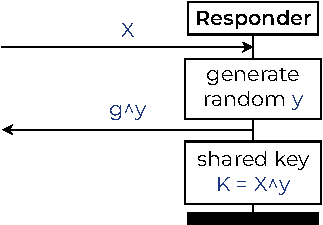
\includegraphics[width=\textwidth]{./figures/lecture_2/dh_r}
            \end{figure}
        \end{column}
        \begin{column}{0.5\textwidth}
            \begin{lstlisting}[style=tamarin, gobble=16]
                builtins: diffie-hellman

                functions: KDF/1

                /* 1. Receive X
                   2. Generate random y
                   3. Send Y = 'g'^y
                   4. Calculate KR */
                rule responder:
                    let
                        Y = 'g'^~y     // 3
                        KR = KDF(X^y)  // 4
                    in
                    [ In(X)            // 1
                    , Fr(~y) ]         // 2
                    -->
                    [ Out(Y) ]         // 3
            \end{lstlisting}
        \end{column}
    \end{columns}
    \vsep
\end{frame}

\begin{frame}[fragile]{Initiator model}
    \begin{columns}
        \begin{column}{0.5\textwidth}
            \begin{figure}
                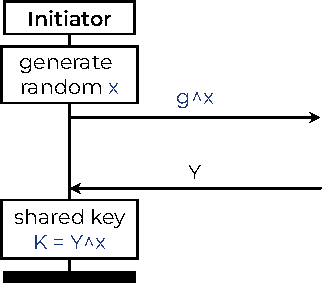
\includegraphics[width=\textwidth]{./figures/lecture_2/dh_i}
            \end{figure}
        \end{column}
        \begin{column}{0.5\textwidth}
            \begin{lstlisting}[style=tamarin, gobble=16]
                /* 1. Generate random x
                   2. Send X = 'g'^x */
                rule initiator_1:
                    let
                      X = 'g'^~x     // 2
                    in
                    [ Fr(~x)         // 1
                    , Fr(~tid) ]
                    -->
                    [ Out(X)         // 2
                    , St_Init_1(~tid, ~x) ]


                /* 3. Receive Y
                   4. Calculate KI */
                rule initiator_2:
                    let
                      KI = KDF(Y^x)  // 4
                    in
                    [ In(Y)          // 3
                    , St_Init_1(~tid, ~x) ]
                    -->
                    [ ]
            \end{lstlisting}
        \end{column}
    \end{columns}
    \vsep
\end{frame}

\begin{frame}[fragile]{Example 2: ISO/IEC}
    \begin{figure}
        \includegraphics<1>[width=.85\textwidth]{./figures/lecture_2/iso_iec}%
        \includegraphics<2>[width=\textwidth]{./figures/lecture_2/iso_iec_0}
    \end{figure}
\end{frame}

\begin{frame}[fragile]{Model}
    \begin{columns}
        \begin{column}{0.4\textwidth}
            \begin{figure}
                \includegraphics<1>[width=\textwidth]
                    {./figures/lecture_2/iso_iec_1}%
                \includegraphics<2>[width=\textwidth]
                    {./figures/lecture_2/iso_iec_2}%
                \includegraphics<3>[width=\textwidth]
                    {./figures/lecture_2/iso_iec_3}%
                \includegraphics<4>[width=\textwidth]
                    {./figures/lecture_2/iso_iec_4}%
                \includegraphics<5>[width=\textwidth]
                    {./figures/lecture_2/iso_iec_5}%
            \end{figure}
        \end{column}
        \begin{column}{0.6\textwidth}
            \begin{onlyenv}<1>
                \begin{lstlisting}[style=tamarin, gobble=20]
                    /* Setup shared keys between $X (variable)
                       and 'T' (fixed trusted server) */
                    rule Setup:
                        [ Fr(~kXT) ]
                        -->
                        [ !SharedKey($X,'T',~kXT) ]

                    /* A initiates the protocol with T */
                    rule A1:
                        [ Fr(~tvpA), Fr(~text1)  ]
                        -->
                        [ Out(<~tvpA,$B,~text1>)
                        , StA1($B,~tvpA) ]
                \end{lstlisting}
            \end{onlyenv}
            \begin{onlyenv}<2>
                \begin{lstlisting}[style=tamarin, gobble=20]
                    /* T receives message from A
                       and responds to A */
                    rule T:
                        let
                          m1 = ~text4
                          m2 = senc(<tvpa,~sesK,B,~text3>,kat)
                          m3 = senc(<~tnT,~sesK,A,~text2>,kbt)
                          tokenTA = <m1,m2,m3>
                        in
                        [ In(<tvpa,B,txt1>)
                        , !SharedKey(A,T,kat)
                        , !SharedKey(B,T,kbt)
                        , Fr(~text2), Fr(~text3), Fr(~text4)
                        , Fr(~sesK), Fr(~tnT) ]
                        -->
                        [ Out(tokenTA) ]
                \end{lstlisting}
            \end{onlyenv}
            \begin{onlyenv}<3>
                \begin{lstlisting}[style=tamarin, gobble=20]
                    /* A receives message from T
                       and responds to B */
                    rule A2:
                        let
                          t2 = senc(<tvpA,sesk,B,text3>,kat)
                          tokenTA  = <t1,t2,t3>
                          m1 = ~text6
                          m2 = t3
                          m3 = senc(<~tnA,B,~text5>,sesk)
                          tokenAB = <m1,m2,m3>
                        in
                        [ In(tokenTA)
                        , !SharedKey(A,T,kat)
                        , StA1(B,tvpA)
                        , Fr(~text5), Fr(~text6), Fr(~tnA) ]
                        -->
                        [ Out(tokenAB)
                        , StA2(A,B,~tnA,sesk) ]
                \end{lstlisting}
            \end{onlyenv}
            \begin{onlyenv}<4>
                \begin{lstlisting}[style=tamarin, gobble=20]
                    /* B receives message from A
                       and responds to A */
                    rule B:
                        let
                          t2 = senc(<tnt,sesk,A,text2>,kbt)
                          t3 = senc(<tna,B,text5>,sesk)
                          tokenAB = <t1,t2,t3>
                          m1 = ~text8
                          m2 = senc(<~tnB,A,~text7>,sesk)
                          tokenBA = <m1,m2>
                        in
                        [ In(tokenAB)
                        , !SharedKey(B,'T',kbt)
                        , Fr(~text7),Fr(~text8),Fr(~tnB) ]
                        -->
                        [ Out(tokenBA) ]
                \end{lstlisting}
            \end{onlyenv}
            \begin{onlyenv}<5>
                \begin{lstlisting}[style=tamarin, gobble=20]
                    /* A receives response from B */
                    rule A3:
                        let
                          t2 = senc(<tnb,A,text7>,sesk)
                          tokenBA = <t1,t2>
                        in
                        [ In(tokenBA)
                        , StA2(A,B,tna,sesk) ]
                        -->
                        [ ]
                \end{lstlisting}
            \end{onlyenv}
        \end{column}
    \end{columns}
    \begin{tikzpicture}[remember picture,overlay]%
        \draw[ultra thick]
            ($(current page.north west)+(6.65cm,0.5cm)$) to
            ($(current page.south west)+(6.65cm,-0.5cm)$);
    \end{tikzpicture}%
\end{frame}

% ---------------------------------------------------------------------------- %

\section*{Summary}

% ---------------------------------------------------------------------------- %

\begin{frame}[fragile]{Summary}
    \begin{itemize}
        \item We now know how to model..
        \begin{itemize}
            \item ..messages as \textbf{terms}
            \item ..cryptographic primitives as \textbf{equational theories}
            \item ..protocol states as \textbf{facts}
            \item ..protocol behavior as \textbf{multiset rewriting rules}
        \end{itemize}
        \item We can now model protocols in a way that Tamarin understands!
        \item In the next lecture, we will learn about modeling
              \textbf{attacker behavior} and express
              \textbf{protocol properties}
    \end{itemize}
\end{frame}

% ---------------------------------------------------------------------------- %
% Reading Material
% ---------------------------------------------------------------------------- %
\begin{frame}[fragile]{Reading material}
    \textbf{Recommended reading}:
        ~\cite[Ch. 3.1.5--3.2.1]{tamarin-book},
        ~\cite[Ch. 3]{cortier2014tutorial}
    \printbibliography[heading=none]
\end{frame}
% ---------------------------------------------------------------------------- %

\end{document}
